\documentclass{standalone}
\usepackage{tikz}
\usepackage{pgfplots}
\usetikzlibrary{shapes.geometric}
\usetikzlibrary{decorations, decorations.text}
%\newcommand{\repeater}[3]{%
 \node ({#1}) at ({#2}) {%
  \begin{tikzpicture}%
   \draw [black,thick] (-.25,0) -- (0,0.5) -- (0.25,0) -- (-0.25,0);%
   \draw [black,thick,domain=-45:225] plot ({0.2*cos(\x)}, {0.5+0.2*sin(\x)});%
   \draw [black,thick,domain=-45:225] plot ({0.4*cos(\x)}, {0.5+0.4*sin(\x)});%
   \node (xxx) at (0,-.2) {{#3}};%
  \end{tikzpicture}%
 } %
}

\newcommand{\activerepeater}[3]{%
 \node ({#1}) at ({#2}) {%
  \begin{tikzpicture}%
   \draw [black,thick] (-.25,0) -- (0,0.5) -- (0.25,0) -- (-0.25,0);%
   \draw [red,thick,domain=-45:225] plot ({0.2*cos(\x)}, {0.5+0.2*sin(\x)});%
   \draw [red,thick,domain=-45:225] plot ({0.4*cos(\x)}, {0.5+0.4*sin(\x)});%
   \node (xxx) at (0,-.2) {{#3}};%
  \end{tikzpicture}%
 } %
}


\newcommand{\user}[3]{%
 \node ({#1}) at ({#2}) {%
  \begin{tikzpicture}%
   \draw [black,fill=black] (-.25,0) -- (0,0.5) -- (0.25,0) -- (-0.25,0);%
   \draw [black,fill=black] (0,.5) circle (.2); %
   \node (xxx) [text width=0.6cm, align=center] at (-.35cm,-.4) {{#3}};%
  \end{tikzpicture}%
 } %
}

\newcommand{\activeuser}[3]{%
 \node ({#1}) at ({#2}) {%
  \begin{tikzpicture}%
   \draw [red,fill=red] (-.25,0) -- (0,0.5) -- (0.25,0) -- (-0.25,0);%
   \draw [red,fill=red] (0,.5) circle (.2); %
   \node (xxx) [text width=0.6cm, align=center] at (-.35cm,-.4) {{#3}};%
  \end{tikzpicture}%
 } %
}

\begin{document}
 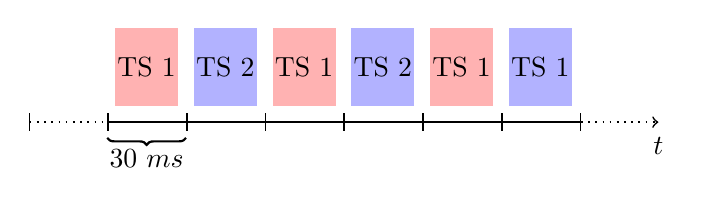
\begin{tikzpicture}
  \draw[|-,dotted, semithick] (-1,-0.2) -- (0,-0.2);
  \draw[|-,semithick] (0,-0.2) -- (1,-0.2);
  \draw[|-,semithick] (1,-0.2) -- (2,-0.2);
  \draw[|-,semithick] (2,-0.2) -- (3,-0.2);
  \draw[|-,semithick] (3,-0.2) -- (4,-0.2);
  \draw[|-,semithick] (4,-0.2) -- (5,-0.2);
  \draw[|-,semithick] (5,-0.2) -- (6,-0.2);
  \draw[|->,dotted,semithick] (6,-0.2) -- (7,-0.2);
  \node at (7, -.5) {$t$};
  \draw [thick,decoration={brace,mirror},decorate] (0,-0.4) -- (1,-0.4) node [pos=0.5, anchor=north,yshift=-0.55] {$30\ ms$}; 
  \fill[red!30] (0.1,0) -- (0.1,1) -- (0.9,1) -- (0.9,0) -- cycle;
  \node at (0.5,0.5) {TS 1};
  \fill[blue!30] (1.1,0) -- (1.1,1) -- (1.9,1) -- (1.9,0) -- cycle;
  \node at (1.5,0.5) {TS 2};
  \fill[red!30] (2.1,0) -- (2.1,1) -- (2.9,1) -- (2.9,0) -- cycle;
  \node at (2.5,0.5) {TS 1};
  \fill[blue!30] (3.1,0) -- (3.1,1) -- (3.9,1) -- (3.9,0) -- cycle;
  \node at (3.5,0.5) {TS 2};
  \fill[red!30] (4.1,0) -- (4.1,1) -- (4.9,1) -- (4.9,0) -- cycle;
  \node at (4.5,0.5) {TS 1};
  \fill[blue!30] (5.1,0) -- (5.1,1) -- (5.9,1) -- (5.9,0) -- cycle;
  \node at (5.5,0.5) {TS 1};  
 \end{tikzpicture}
\end{document}
